\section{Methodology}
\label{sec:methodology}

Figure~\ref{fig:workflow} summarizes the implemented adaptation and its evaluation.
The method modifies the input representation while keeping the backbone generator
fixed. It does not learn new weights, infer a joint reconstruction from several
patent views, or condition generation on captions.

\begin{figure*}[t]
\centering
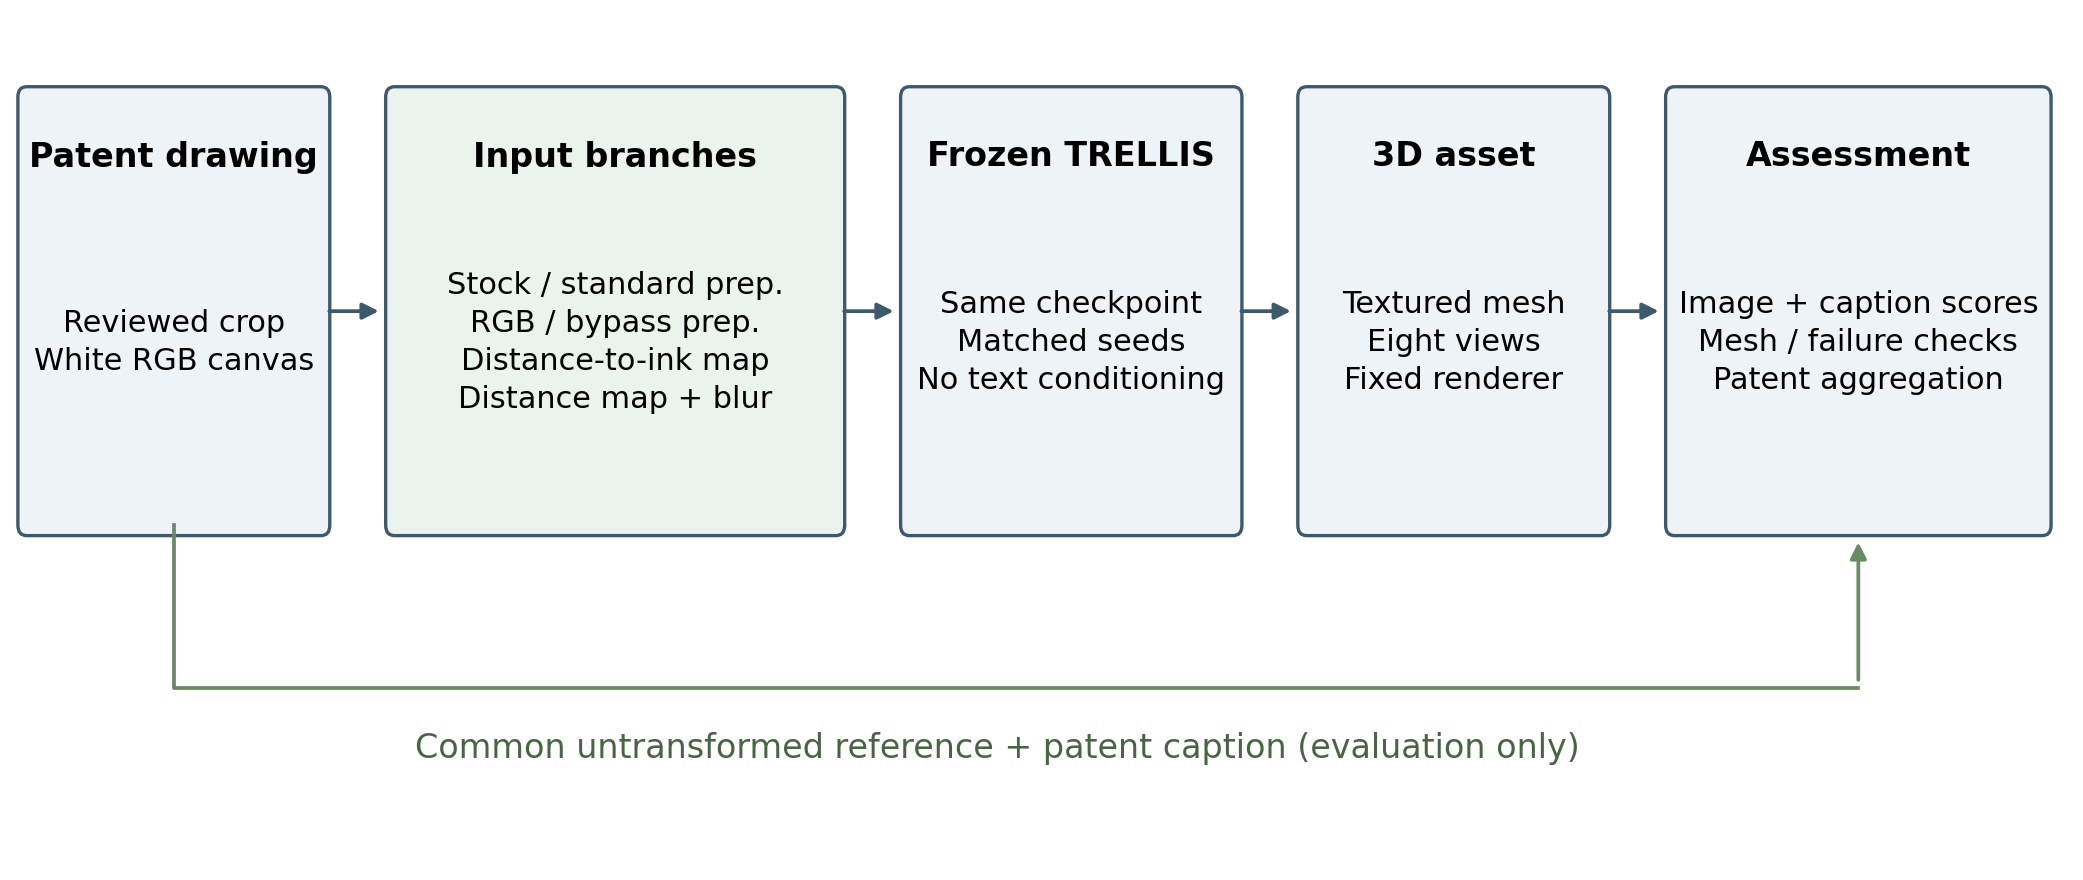
\includegraphics[width=\textwidth]{figures/workflow.png}
\caption{Implemented workflow. A reviewed patent crop supplies both the generator
input and a common untransformed reference for evaluation. Controlled branches
isolate standard preprocessing, background-removal bypass, distance mapping,
and smoothing. The same frozen TRELLIS backbone and seeds are used across branches.
Captions enter evaluation only. The diagram specifies the experiment, not a
claim of measured improvement.}
\label{fig:workflow}
\end{figure*}

\subsection{Sketch-Preserving Input Representation}
Let $I$ denote an RGB patent image and $C(I)$ a reviewed crop containing one
figure. A deterministic operator $P$ preserves aspect ratio and places the crop
on a white square canvas, giving $J=P(C(I))$. The same $J$ is used across all
configurations. Reviewing the crop prevents labels or unrelated figures from
being silently treated as a single object.

We identify dark ink with a grayscale threshold $\tau$:
\begin{equation}
 M(x)=\mathbb{1}[\operatorname{gray}(J(x))\leq\tau].
\end{equation}
Unlike the evaluation-mask procedure, the adaptation does not apply opening or
small-component removal, because thin strokes and disconnected marks may carry
structural information. Blank or uniform masks are rejected for inspection.
The representation assumes dark linework on a light background and does not
attempt to decide whether dashed lines indicate visible or hidden surfaces.

\subsection{Distance-Based Structural Adaptation}
The distance to the nearest detected ink pixel is
\begin{equation}
 d_M(x)=\min_{y:M(y)=1}\|x-y\|_2.
\end{equation}
For support width $\sigma_d>0$, we form
\begin{equation}
 B_{\sigma_d}(x)=\exp\left[-\frac{d_M(x)^2}{2\sigma_d^2}\right].
\end{equation}
The image supplied to the generator is $A_d=1-B_{\sigma_d}$, replicated across
RGB channels. The optional smoothed version is
$A_{d,g}=1-(G_{\sigma_g}*B_{\sigma_d})$, where $G_{\sigma_g}$ is a Gaussian
kernel. Both maps are quantized to the image range. Increasing support width
expands influence around ink; smoothing changes local transitions. Neither
operation supplies missing depth or establishes calibrated boundary probabilities.
Figure~\ref{fig:input_ablation} shows actual prepared inputs.

\subsection{Frozen Generator and Controlled Branches}
We use TRELLIS~\cite{xiang2025trellis} as the backbone generator $G_\theta$.
For representation $A_v$ and seed $s$, the output is
\begin{equation}
 \mathcal O_{i,v,s}=G_\theta(A_v(J_i);s,b_v),
\end{equation}
where $b_v$ specifies whether the backbone's standard input preprocessing is
enabled. The stock branch uses $A_v(J)=J$ with preprocessing enabled; bypass
uses the same pixels with preprocessing disabled. Distance and distance-plus-blur
also disable that preprocessing, isolating representation changes from
background removal. Identical seeds are paired across branches. Architecture,
checkpoint, and export settings are held fixed; implementation details are in
Section~\ref{sec:implementation}.

\subsection{Paired Assessment}
We compare every rendered reconstruction with the same untransformed reference
$J_i$, not its adapted map. Image measurements assess structural, perceptual,
and semantic agreement; mesh statistics characterize the exported representation.
For metric $m$, view scores are averaged within each output, seeds within each
drawing, and drawings within each patent:
\begin{equation}
 M_{p,v}=\frac{1}{|\mathcal I_p|}\sum_{i\in\mathcal I_p}
 \frac{1}{|\mathcal S|}\sum_{s\in\mathcal S}
 \frac{1}{|\mathcal V_{i,v,s}|}\sum_{a\in\mathcal V_{i,v,s}}m_{i,v,s,a}.
\end{equation}
We report the mean and sample standard deviation across patents. For paired
changes, the analysis uses the common finite-score sample set across all
requested branches and seeds, and resamples patent-level differences.
Failure counts are reported separately because complete-case scores alone can
hide unsuccessful runs. The historical archive contains one recorded output per
drawing and is analyzed separately from this matched protocol.
